\documentclass[twoside]{book}

% Packages required by doxygen
\usepackage{calc}
\usepackage{doxygen}
\usepackage{graphicx}
\usepackage[utf8]{inputenc}
\usepackage{makeidx}
\usepackage{multicol}
\usepackage{multirow}
\usepackage{textcomp}
\usepackage[table]{xcolor}

% Font selection
\usepackage[T1]{fontenc}
\usepackage{mathptmx}
\usepackage[scaled=.90]{helvet}
\usepackage{courier}
\usepackage{amssymb}
\usepackage{sectsty}
\renewcommand{\familydefault}{\sfdefault}
\allsectionsfont{%
  \fontseries{bc}\selectfont%
  \color{darkgray}%
}
\renewcommand{\DoxyLabelFont}{%
  \fontseries{bc}\selectfont%
  \color{darkgray}%
}

% Page & text layout
\usepackage{geometry}
\geometry{%
  a4paper,%
  top=2.5cm,%
  bottom=2.5cm,%
  left=2.5cm,%
  right=2.5cm%
}
\tolerance=750
\hfuzz=15pt
\hbadness=750
\setlength{\emergencystretch}{15pt}
\setlength{\parindent}{0cm}
\setlength{\parskip}{0.2cm}
\makeatletter
\renewcommand{\paragraph}{%
  \@startsection{paragraph}{4}{0ex}{-1.0ex}{1.0ex}{%
    \normalfont\normalsize\bfseries\SS@parafont%
  }%
}
\renewcommand{\subparagraph}{%
  \@startsection{subparagraph}{5}{0ex}{-1.0ex}{1.0ex}{%
    \normalfont\normalsize\bfseries\SS@subparafont%
  }%
}
\makeatother

% Headers & footers
\usepackage{fancyhdr}
\pagestyle{fancyplain}
\fancyhead[LE]{\fancyplain{}{\bfseries\thepage}}
\fancyhead[CE]{\fancyplain{}{}}
\fancyhead[RE]{\fancyplain{}{\bfseries\leftmark}}
\fancyhead[LO]{\fancyplain{}{\bfseries\rightmark}}
\fancyhead[CO]{\fancyplain{}{}}
\fancyhead[RO]{\fancyplain{}{\bfseries\thepage}}
\fancyfoot[LE]{\fancyplain{}{}}
\fancyfoot[CE]{\fancyplain{}{}}
\fancyfoot[RE]{\fancyplain{}{\bfseries\scriptsize Generated on Mon Feb 5 2018 19\-:14\-:56 for My Project by Doxygen }}
\fancyfoot[LO]{\fancyplain{}{\bfseries\scriptsize Generated on Mon Feb 5 2018 19\-:14\-:56 for My Project by Doxygen }}
\fancyfoot[CO]{\fancyplain{}{}}
\fancyfoot[RO]{\fancyplain{}{}}
\renewcommand{\footrulewidth}{0.4pt}
\renewcommand{\chaptermark}[1]{%
  \markboth{#1}{}%
}
\renewcommand{\sectionmark}[1]{%
  \markright{\thesection\ #1}%
}

% Indices & bibliography
\usepackage{natbib}
\usepackage[titles]{tocloft}
\setcounter{tocdepth}{3}
\setcounter{secnumdepth}{5}
\makeindex

% Hyperlinks (required, but should be loaded last)
\usepackage{ifpdf}
\ifpdf
  \usepackage[pdftex,pagebackref=true]{hyperref}
\else
  \usepackage[ps2pdf,pagebackref=true]{hyperref}
\fi
\hypersetup{%
  colorlinks=true,%
  linkcolor=blue,%
  citecolor=blue,%
  unicode%
}

% Custom commands
\newcommand{\clearemptydoublepage}{%
  \newpage{\pagestyle{empty}\cleardoublepage}%
}


%===== C O N T E N T S =====

\begin{document}

% Titlepage & ToC
\hypersetup{pageanchor=false}
\pagenumbering{roman}
\begin{titlepage}
\vspace*{7cm}
\begin{center}%
{\Large My Project }\\
\vspace*{1cm}
{\large Generated by Doxygen 1.8.6}\\
\vspace*{0.5cm}
{\small Mon Feb 5 2018 19:14:56}\\
\end{center}
\end{titlepage}
\clearemptydoublepage
\tableofcontents
\clearemptydoublepage
\pagenumbering{arabic}
\hypersetup{pageanchor=true}

%--- Begin generated contents ---
\chapter{Class Index}
\section{Class List}
Here are the classes, structs, unions and interfaces with brief descriptions\-:\begin{DoxyCompactList}
\item\contentsline{section}{\hyperlink{class_document}{Document} }{\pageref{class_document}}{}
\item\contentsline{section}{\hyperlink{class_graphic_editor}{Graphic\-Editor} }{\pageref{class_graphic_editor}}{}
\item\contentsline{section}{\hyperlink{class_graphic_element}{Graphic\-Element} }{\pageref{class_graphic_element}}{}
\item\contentsline{section}{\hyperlink{class_line}{Line} }{\pageref{class_line}}{}
\item\contentsline{section}{\hyperlink{class_square}{Square} }{\pageref{class_square}}{}
\item\contentsline{section}{\hyperlink{class_triangle}{Triangle} }{\pageref{class_triangle}}{}
\end{DoxyCompactList}

\chapter{File Index}
\section{File List}
Here is a list of all files with brief descriptions\-:\begin{DoxyCompactList}
\item\contentsline{section}{\hyperlink{header_8h}{header.\-h} }{\pageref{header_8h}}{}
\item\contentsline{section}{\hyperlink{main_8cpp}{main.\-cpp} }{\pageref{main_8cpp}}{}
\item\contentsline{section}{\hyperlink{version_8h}{version.\-h} }{\pageref{version_8h}}{}
\end{DoxyCompactList}

\chapter{Class Documentation}
\hypertarget{structis__container}{\section{is\-\_\-container$<$ T $>$ Struct Template Reference}
\label{structis__container}\index{is\-\_\-container$<$ T $>$@{is\-\_\-container$<$ T $>$}}
}


{\ttfamily \#include $<$type\-\_\-check.\-h$>$}

\subsection*{Static Public Attributes}
\begin{DoxyCompactItemize}
\item 
static constexpr bool \hyperlink{structis__container_abe72bf896680aa10340ccf08a5d293c7}{value} = has\-\_\-iterator$<$T$>$(nullptr)
\end{DoxyCompactItemize}


\subsection{Member Data Documentation}
\hypertarget{structis__container_abe72bf896680aa10340ccf08a5d293c7}{\index{is\-\_\-container@{is\-\_\-container}!value@{value}}
\index{value@{value}!is_container@{is\-\_\-container}}
\subsubsection[{value}]{\setlength{\rightskip}{0pt plus 5cm}template$<$typename T $>$ constexpr bool {\bf is\-\_\-container}$<$ T $>$\-::value = has\-\_\-iterator$<$T$>$(nullptr)\hspace{0.3cm}{\ttfamily [static]}}}\label{structis__container_abe72bf896680aa10340ccf08a5d293c7}


The documentation for this struct was generated from the following file\-:\begin{DoxyCompactItemize}
\item 
\hyperlink{type__check_8h}{type\-\_\-check.\-h}\end{DoxyCompactItemize}

\hypertarget{struct_same_type_check}{\section{Same\-Type\-Check$<$ N, T, Args $>$ Struct Template Reference}
\label{struct_same_type_check}\index{Same\-Type\-Check$<$ N, T, Args $>$@{Same\-Type\-Check$<$ N, T, Args $>$}}
}


{\ttfamily \#include $<$type\-\_\-check.\-h$>$}

\subsection*{Public Types}
\begin{DoxyCompactItemize}
\item 
typedef T \hyperlink{struct_same_type_check_a2bd1b23b5f7e5f14acc5a64274651adb}{type}
\end{DoxyCompactItemize}
\subsection*{Static Public Attributes}
\begin{DoxyCompactItemize}
\item 
static constexpr bool \hyperlink{struct_same_type_check_a90fe116ef2512e49fc0065e1c9ccf302}{value}
\end{DoxyCompactItemize}


\subsection{Member Typedef Documentation}
\hypertarget{struct_same_type_check_a2bd1b23b5f7e5f14acc5a64274651adb}{\index{Same\-Type\-Check@{Same\-Type\-Check}!type@{type}}
\index{type@{type}!SameTypeCheck@{Same\-Type\-Check}}
\subsubsection[{type}]{\setlength{\rightskip}{0pt plus 5cm}template$<$size\-\_\-t N, typename T , typename... Args$>$ typedef T {\bf Same\-Type\-Check}$<$ N, T, Args $>$\-::{\bf type}}}\label{struct_same_type_check_a2bd1b23b5f7e5f14acc5a64274651adb}


\subsection{Member Data Documentation}
\hypertarget{struct_same_type_check_a90fe116ef2512e49fc0065e1c9ccf302}{\index{Same\-Type\-Check@{Same\-Type\-Check}!value@{value}}
\index{value@{value}!SameTypeCheck@{Same\-Type\-Check}}
\subsubsection[{value}]{\setlength{\rightskip}{0pt plus 5cm}template$<$size\-\_\-t N, typename T , typename... Args$>$ constexpr bool {\bf Same\-Type\-Check}$<$ N, T, Args $>$\-::value\hspace{0.3cm}{\ttfamily [static]}}}\label{struct_same_type_check_a90fe116ef2512e49fc0065e1c9ccf302}
{\bfseries Initial value\-:}
\begin{DoxyCode}
= std::is\_same<T,\textcolor{keyword}{typename} \hyperlink{struct_same_type_check}{SameTypeCheck}<\textcolor{keyword}{sizeof}...(Args)-1,Args...>::
      \hyperlink{struct_same_type_check_a2bd1b23b5f7e5f14acc5a64274651adb}{type}>::\hyperlink{struct_same_type_check_a90fe116ef2512e49fc0065e1c9ccf302}{value}
                                  && \hyperlink{struct_same_type_check}{SameTypeCheck}<\textcolor{keyword}{sizeof}...(Args)-1,Args...>
      \hyperlink{struct_same_type_check_a90fe116ef2512e49fc0065e1c9ccf302}{::value}
\end{DoxyCode}


The documentation for this struct was generated from the following file\-:\begin{DoxyCompactItemize}
\item 
\hyperlink{type__check_8h}{type\-\_\-check.\-h}\end{DoxyCompactItemize}

\hypertarget{struct_same_type_check_3_010_00_01_t_01_4}{\section{Same\-Type\-Check$<$ 0, T $>$ Struct Template Reference}
\label{struct_same_type_check_3_010_00_01_t_01_4}\index{Same\-Type\-Check$<$ 0, T $>$@{Same\-Type\-Check$<$ 0, T $>$}}
}


{\ttfamily \#include $<$type\-\_\-check.\-h$>$}

\subsection*{Public Types}
\begin{DoxyCompactItemize}
\item 
typedef T \hyperlink{struct_same_type_check_3_010_00_01_t_01_4_afc0f35b366f82eb7f0051a7de6c9070f}{type}
\end{DoxyCompactItemize}
\subsection*{Static Public Attributes}
\begin{DoxyCompactItemize}
\item 
static constexpr bool \hyperlink{struct_same_type_check_3_010_00_01_t_01_4_a0faa450f2776529e025404d2d16c0e7e}{value} = true
\end{DoxyCompactItemize}


\subsection{Member Typedef Documentation}
\hypertarget{struct_same_type_check_3_010_00_01_t_01_4_afc0f35b366f82eb7f0051a7de6c9070f}{\index{Same\-Type\-Check$<$ 0, T $>$@{Same\-Type\-Check$<$ 0, T $>$}!type@{type}}
\index{type@{type}!SameTypeCheck< 0, T >@{Same\-Type\-Check$<$ 0, T $>$}}
\subsubsection[{type}]{\setlength{\rightskip}{0pt plus 5cm}template$<$typename T $>$ typedef T {\bf Same\-Type\-Check}$<$ 0, T $>$\-::{\bf type}}}\label{struct_same_type_check_3_010_00_01_t_01_4_afc0f35b366f82eb7f0051a7de6c9070f}


\subsection{Member Data Documentation}
\hypertarget{struct_same_type_check_3_010_00_01_t_01_4_a0faa450f2776529e025404d2d16c0e7e}{\index{Same\-Type\-Check$<$ 0, T $>$@{Same\-Type\-Check$<$ 0, T $>$}!value@{value}}
\index{value@{value}!SameTypeCheck< 0, T >@{Same\-Type\-Check$<$ 0, T $>$}}
\subsubsection[{value}]{\setlength{\rightskip}{0pt plus 5cm}template$<$typename T $>$ constexpr bool {\bf Same\-Type\-Check}$<$ 0, T $>$\-::value = true\hspace{0.3cm}{\ttfamily [static]}}}\label{struct_same_type_check_3_010_00_01_t_01_4_a0faa450f2776529e025404d2d16c0e7e}


The documentation for this struct was generated from the following file\-:\begin{DoxyCompactItemize}
\item 
\hyperlink{type__check_8h}{type\-\_\-check.\-h}\end{DoxyCompactItemize}

\hypertarget{struct_tuple_printer}{\section{Tuple\-Printer$<$ Tuple, N $>$ Struct Template Reference}
\label{struct_tuple_printer}\index{Tuple\-Printer$<$ Tuple, N $>$@{Tuple\-Printer$<$ Tuple, N $>$}}
}


{\ttfamily \#include $<$print.\-h$>$}

\subsection*{Static Public Member Functions}
\begin{DoxyCompactItemize}
\item 
static void \hyperlink{struct_tuple_printer_aaf76573f278205ba63759d5dbe3f408c}{print} (const Tuple \&t)
\end{DoxyCompactItemize}


\subsection{Member Function Documentation}
\hypertarget{struct_tuple_printer_aaf76573f278205ba63759d5dbe3f408c}{\index{Tuple\-Printer@{Tuple\-Printer}!print@{print}}
\index{print@{print}!TuplePrinter@{Tuple\-Printer}}
\subsubsection[{print}]{\setlength{\rightskip}{0pt plus 5cm}template$<$typename Tuple , std\-::size\-\_\-t N$>$ static void {\bf Tuple\-Printer}$<$ Tuple, N $>$\-::print (
\begin{DoxyParamCaption}
\item[{const Tuple \&}]{t}
\end{DoxyParamCaption}
)\hspace{0.3cm}{\ttfamily [inline]}, {\ttfamily [static]}}}\label{struct_tuple_printer_aaf76573f278205ba63759d5dbe3f408c}


The documentation for this struct was generated from the following file\-:\begin{DoxyCompactItemize}
\item 
\hyperlink{print_8h}{print.\-h}\end{DoxyCompactItemize}

\hypertarget{struct_tuple_printer_3_01_tuple_00_011_01_4}{\section{Tuple\-Printer$<$ Tuple, 1 $>$ Struct Template Reference}
\label{struct_tuple_printer_3_01_tuple_00_011_01_4}\index{Tuple\-Printer$<$ Tuple, 1 $>$@{Tuple\-Printer$<$ Tuple, 1 $>$}}
}


{\ttfamily \#include $<$print.\-h$>$}

\subsection*{Static Public Member Functions}
\begin{DoxyCompactItemize}
\item 
static void \hyperlink{struct_tuple_printer_3_01_tuple_00_011_01_4_af4ab0b518a1d2927e949c817aa6b7266}{print} (const Tuple \&t)
\end{DoxyCompactItemize}


\subsection{Member Function Documentation}
\hypertarget{struct_tuple_printer_3_01_tuple_00_011_01_4_af4ab0b518a1d2927e949c817aa6b7266}{\index{Tuple\-Printer$<$ Tuple, 1 $>$@{Tuple\-Printer$<$ Tuple, 1 $>$}!print@{print}}
\index{print@{print}!TuplePrinter< Tuple, 1 >@{Tuple\-Printer$<$ Tuple, 1 $>$}}
\subsubsection[{print}]{\setlength{\rightskip}{0pt plus 5cm}template$<$typename Tuple $>$ static void {\bf Tuple\-Printer}$<$ Tuple, 1 $>$\-::print (
\begin{DoxyParamCaption}
\item[{const Tuple \&}]{t}
\end{DoxyParamCaption}
)\hspace{0.3cm}{\ttfamily [inline]}, {\ttfamily [static]}}}\label{struct_tuple_printer_3_01_tuple_00_011_01_4_af4ab0b518a1d2927e949c817aa6b7266}


The documentation for this struct was generated from the following file\-:\begin{DoxyCompactItemize}
\item 
\hyperlink{print_8h}{print.\-h}\end{DoxyCompactItemize}

\chapter{File Documentation}
\hypertarget{main_8cpp}{\section{main.\-cpp File Reference}
\label{main_8cpp}\index{main.\-cpp@{main.\-cpp}}
}
{\ttfamily \#include \char`\"{}header.\-h\char`\"{}}\\*
{\ttfamily \#include $<$memory$>$}\\*
Include dependency graph for main.\-cpp\-:
\nopagebreak
\begin{figure}[H]
\begin{center}
\leavevmode
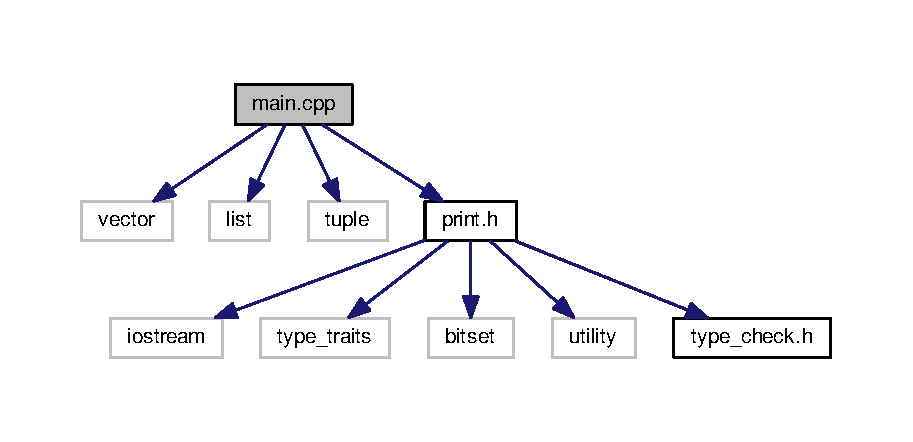
\includegraphics[width=237pt]{main_8cpp__incl}
\end{center}
\end{figure}
\subsection*{Classes}
\begin{DoxyCompactItemize}
\item 
class \hyperlink{class_graphic_editor}{Graphic\-Editor}
\end{DoxyCompactItemize}
\subsection*{Functions}
\begin{DoxyCompactItemize}
\item 
int \hyperlink{main_8cpp_ae66f6b31b5ad750f1fe042a706a4e3d4}{main} ()
\end{DoxyCompactItemize}


\subsection{Function Documentation}
\hypertarget{main_8cpp_ae66f6b31b5ad750f1fe042a706a4e3d4}{\index{main.\-cpp@{main.\-cpp}!main@{main}}
\index{main@{main}!main.cpp@{main.\-cpp}}
\subsubsection[{main}]{\setlength{\rightskip}{0pt plus 5cm}int main (
\begin{DoxyParamCaption}
{}
\end{DoxyParamCaption}
)}}\label{main_8cpp_ae66f6b31b5ad750f1fe042a706a4e3d4}

\hypertarget{print_8h}{\section{print.\-h File Reference}
\label{print_8h}\index{print.\-h@{print.\-h}}
}
{\ttfamily \#include $<$iostream$>$}\\*
{\ttfamily \#include $<$type\-\_\-traits$>$}\\*
{\ttfamily \#include $<$bitset$>$}\\*
{\ttfamily \#include $<$utility$>$}\\*
{\ttfamily \#include \char`\"{}type\-\_\-check.\-h\char`\"{}}\\*
Include dependency graph for print.\-h\-:
\nopagebreak
\begin{figure}[H]
\begin{center}
\leavevmode
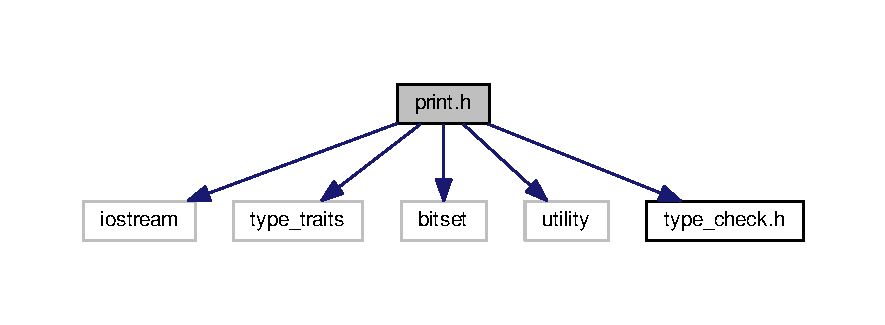
\includegraphics[width=350pt]{print_8h__incl}
\end{center}
\end{figure}
This graph shows which files directly or indirectly include this file\-:
\nopagebreak
\begin{figure}[H]
\begin{center}
\leavevmode
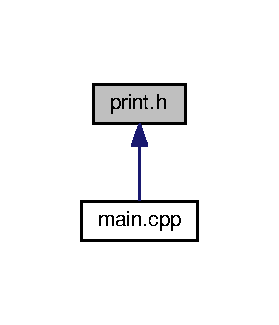
\includegraphics[width=134pt]{print_8h__dep__incl}
\end{center}
\end{figure}
\subsection*{Classes}
\begin{DoxyCompactItemize}
\item 
struct \hyperlink{struct_tuple_printer}{Tuple\-Printer$<$ Tuple, N $>$}
\item 
struct \hyperlink{struct_tuple_printer_3_01_tuple_00_011_01_4}{Tuple\-Printer$<$ Tuple, 1 $>$}
\end{DoxyCompactItemize}
\subsection*{Functions}
\begin{DoxyCompactItemize}
\item 
{\footnotesize template$<$typename Integral , typename std\-::enable\-\_\-if$<$ std\-::is\-\_\-integral$<$ Integral $>$\-::value, Integral $\ast$ $>$\-::type  = nullptr$>$ }\\void \hyperlink{print_8h_ae115ec29a208f2abe4c9caa427a2a67a}{print\-\_\-ip} (const Integral \&value)
\item 
{\footnotesize template$<$typename Container , typename std\-::enable\-\_\-if$<$ is\-\_\-container$<$ Container $>$\-::value \&\&!std\-::is\-\_\-same$<$ Container, std\-::string $>$\-::value, Container $\ast$ $>$\-::type  = nullptr$>$ }\\void \hyperlink{print_8h_a8ed4d78a6c98462b99031e0eceb0681a}{print\-\_\-ip} (const Container \&container)
\item 
{\footnotesize template$<$typename... Args, typename std\-::enable\-\_\-if$<$ Same\-Type\-Check$<$ sizeof...(\-Args), Args...$>$\-::value, void $\ast$ $>$\-::type  = nullptr$>$ }\\void \hyperlink{print_8h_a9d66204a843e107d6a46614e62d86a25}{print\-\_\-ip} (const std\-::tuple$<$ Args...$>$ \&t)
\end{DoxyCompactItemize}


\subsection{Function Documentation}
\hypertarget{print_8h_ae115ec29a208f2abe4c9caa427a2a67a}{\index{print.\-h@{print.\-h}!print\-\_\-ip@{print\-\_\-ip}}
\index{print\-\_\-ip@{print\-\_\-ip}!print.h@{print.\-h}}
\subsubsection[{print\-\_\-ip}]{\setlength{\rightskip}{0pt plus 5cm}template$<$typename Integral , typename std\-::enable\-\_\-if$<$ std\-::is\-\_\-integral$<$ Integral $>$\-::value, Integral $\ast$ $>$\-::type  = nullptr$>$ void print\-\_\-ip (
\begin{DoxyParamCaption}
\item[{const Integral \&}]{value}
\end{DoxyParamCaption}
)}}\label{print_8h_ae115ec29a208f2abe4c9caa427a2a67a}
Функция печати ip-\/адреса для целочисленных типов 
\begin{DoxyTemplParams}{Template Parameters}
{\em Integral} & -\/ целочисленный тип \\
\hline
\end{DoxyTemplParams}

\begin{DoxyParams}{Parameters}
{\em value} & -\/ значение, передаваемое в функцию \\
\hline
\end{DoxyParams}
\hypertarget{print_8h_a8ed4d78a6c98462b99031e0eceb0681a}{\index{print.\-h@{print.\-h}!print\-\_\-ip@{print\-\_\-ip}}
\index{print\-\_\-ip@{print\-\_\-ip}!print.h@{print.\-h}}
\subsubsection[{print\-\_\-ip}]{\setlength{\rightskip}{0pt plus 5cm}template$<$typename Container , typename std\-::enable\-\_\-if$<$ is\-\_\-container$<$ Container $>$\-::value \&\&!std\-::is\-\_\-same$<$ Container, std\-::string $>$\-::value, Container $\ast$ $>$\-::type  = nullptr$>$ void print\-\_\-ip (
\begin{DoxyParamCaption}
\item[{const Container \&}]{container}
\end{DoxyParamCaption}
)}}\label{print_8h_a8ed4d78a6c98462b99031e0eceb0681a}
Функция печати ip-\/адреса для целочисленных типов 
\begin{DoxyTemplParams}{Template Parameters}
{\em Container} & -\/ тип контейнера \\
\hline
\end{DoxyTemplParams}

\begin{DoxyParams}{Parameters}
{\em container} & -\/ объект контейнера \\
\hline
\end{DoxyParams}
\hypertarget{print_8h_a9d66204a843e107d6a46614e62d86a25}{\index{print.\-h@{print.\-h}!print\-\_\-ip@{print\-\_\-ip}}
\index{print\-\_\-ip@{print\-\_\-ip}!print.h@{print.\-h}}
\subsubsection[{print\-\_\-ip}]{\setlength{\rightskip}{0pt plus 5cm}template$<$typename... Args, typename std\-::enable\-\_\-if$<$ Same\-Type\-Check$<$ sizeof...(\-Args), Args...$>$\-::value, void $\ast$ $>$\-::type  = nullptr$>$ void print\-\_\-ip (
\begin{DoxyParamCaption}
\item[{const std\-::tuple$<$ Args...$>$ \&}]{tp}
\end{DoxyParamCaption}
)}}\label{print_8h_a9d66204a843e107d6a46614e62d86a25}
Функция печати ip-\/адреса для кортежа 
\begin{DoxyTemplParams}{Template Parameters}
{\em Args} & -\/ типы в кортеже \\
\hline
\end{DoxyTemplParams}

\begin{DoxyParams}{Parameters}
{\em t} & -\/ объект кортежа \\
\hline
\end{DoxyParams}

\hypertarget{type__check_8h}{\section{type\-\_\-check.\-h File Reference}
\label{type__check_8h}\index{type\-\_\-check.\-h@{type\-\_\-check.\-h}}
}
This graph shows which files directly or indirectly include this file\-:
\nopagebreak
\begin{figure}[H]
\begin{center}
\leavevmode
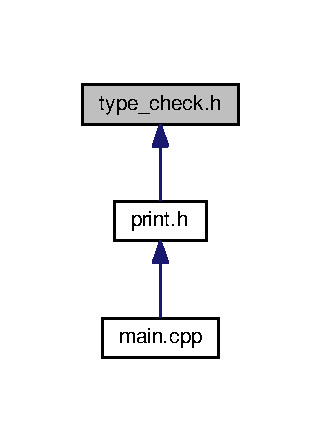
\includegraphics[width=154pt]{type__check_8h__dep__incl}
\end{center}
\end{figure}
\subsection*{Classes}
\begin{DoxyCompactItemize}
\item 
struct \hyperlink{structis__container}{is\-\_\-container$<$ T $>$}
\item 
struct \hyperlink{struct_same_type_check}{Same\-Type\-Check$<$ N, T, Args $>$}
\item 
struct \hyperlink{struct_same_type_check_3_010_00_01_t_01_4}{Same\-Type\-Check$<$ 0, T $>$}
\end{DoxyCompactItemize}

\hypertarget{version_8h}{\section{version.\-h File Reference}
\label{version_8h}\index{version.\-h@{version.\-h}}
}
\subsection*{Macros}
\begin{DoxyCompactItemize}
\item 
\#define \hyperlink{version_8h_a4a5fc96a4bdd7d68ed99ccce9ca2e77e}{P\-R\-O\-J\-E\-C\-T\-\_\-\-V\-E\-R\-S\-I\-O\-N\-\_\-\-P\-A\-T\-C\-H}~44
\end{DoxyCompactItemize}


\subsection{Macro Definition Documentation}
\hypertarget{version_8h_a4a5fc96a4bdd7d68ed99ccce9ca2e77e}{\index{version.\-h@{version.\-h}!P\-R\-O\-J\-E\-C\-T\-\_\-\-V\-E\-R\-S\-I\-O\-N\-\_\-\-P\-A\-T\-C\-H@{P\-R\-O\-J\-E\-C\-T\-\_\-\-V\-E\-R\-S\-I\-O\-N\-\_\-\-P\-A\-T\-C\-H}}
\index{P\-R\-O\-J\-E\-C\-T\-\_\-\-V\-E\-R\-S\-I\-O\-N\-\_\-\-P\-A\-T\-C\-H@{P\-R\-O\-J\-E\-C\-T\-\_\-\-V\-E\-R\-S\-I\-O\-N\-\_\-\-P\-A\-T\-C\-H}!version.h@{version.\-h}}
\subsubsection[{P\-R\-O\-J\-E\-C\-T\-\_\-\-V\-E\-R\-S\-I\-O\-N\-\_\-\-P\-A\-T\-C\-H}]{\setlength{\rightskip}{0pt plus 5cm}\#define P\-R\-O\-J\-E\-C\-T\-\_\-\-V\-E\-R\-S\-I\-O\-N\-\_\-\-P\-A\-T\-C\-H~44}}\label{version_8h_a4a5fc96a4bdd7d68ed99ccce9ca2e77e}

%--- End generated contents ---

% Index
\newpage
\phantomsection
\addcontentsline{toc}{chapter}{Index}
\printindex

\end{document}
